\chapter{Newton's Laws}

\pagestyle{fancy}
\fancyhf{}
\fancyhead[OC]{\leftmark}
\fancyhead[EC]{\rightmark}
%\renewcommand{\footrulewidth}{1pt}
\cfoot{\thepage}

\section{Key Concepts and Formulae}


\begin{enumerate}
\item For problems involving dynamics of the system, check if the situation is an analogy of simple harmonic motion(SHM). If the situation can be modeled to SHM, we can easily find some unknown parameters required to solve the problem. For example, the system  under a force proportional to x(displacement) can be compared with SHM. 

\item When a body is supposed to leave a surface, ensure that the net normal force on the body is zero. 

\item momentum equation vs. energy equation for scattering problems

\item In a perfectly elastic collision, the colliding particle scatter by double the initial angle, unless the collision is head-on. figure..  

\end{enumerate}

\section{Bridging Problem}
When viewed from the side, the cone in the figure subtends an angle $2\theta$ at its tip. A block of mass $m$ is connected to the tip by a massless string and moves in a horizontal circle of radius $R$ around the surface. If the initial speed is $v_0$ and if the coefficient of kinetic friction between the block and the cone is $\mu$, how much time does it take the block to stop? \hfill \textsl{Morin 3.70}

\begin{figure}[hbt]
    \centering
    \includesvg[width = 0.3\textwidth]{figures/ch2/cone.svg}
\end{figure}

\textsc{Solution:}\\
First draw a free body diagram of the block indicating all forces, their directions and choice of axes. Assume the block is moving into the plane of figure. Frictional force always opposes motion and hence points out of the plane of the figure. ($\odot$ signifies out of the plane of figure and $\otimes$ into the plane.)\\
Now we need to find the value of $f_r$ and for that we need the value of $N$ since $f_r=\mu N$. Before using Newton's Laws to find $N$, assess the values of $a_x$ and $a_y$.
\begin{figure}[hbt]
    \centering
    \includesvg[width = 0.3\textwidth]{figures/ch2/cone_fbd.svg}
\end{figure}
\begin{align*}
a_y&=0 \qquad \because\text{no vertical motion}\\
a_x&=\frac{v^2}{R} \qquad \because\text{circular motion}
\end{align*}
Using Newton's Laws,
\begin{align}
 \sum F_y&=ma_y \nonumber\\
T\cos\theta + N\sin\theta - mg&=0 \label{eq31}\\
\sum F_x &= ma_x \nonumber\\
T\sin\theta - N\cos\theta &= \ddfrac{mv^2}{R}\label{eq32}
\end{align}
Eliminating $T$ from \eqref{eq31} and \eqref{eq32} and solving for $N$, we get,
\begin{equation}
N=mg\sin\theta - \ddfrac{mv^2\cos\theta}{R} \label{eq33}
\end{equation}
As discussed earlier, friction opposes the motion and causes the block to slow down over time. Mathematically,
\begin{equation*}
m\ddfrac{\diff v}{\diff t}=-\mu N
\end{equation*}
Using \eqref{eq33}, we get
\begin{equation*}
\ddfrac{\diff v}{gR\tan\theta - v^2}=-\ddfrac{\mu \cos \theta}{R}\diff t
\end{equation*}
If the total time taken by the block to stop is $\tau$. use the limits
\begin{align*}
v&=v_0 \quad \text{at} \quad t=0\\
v&=0 \quad \text{at} \quad t=\tau
\end{align*}
\begin{align*}
\int_{v_0}^0 \ddfrac{\diff v}{gR\tan \theta - v^2}&=-\int_0^\tau \frac{\mu \cos \theta}{R} \diff t\\
-\frac{\mu\cos\theta}{R}\tau&= \frac{1}{2\sqrt{gR\tan\theta}}\biggl|\ln \frac{\sqrt{gR\tan\theta}+v}{\sqrt{gR\tan\theta}-v}\biggr|_{v_0}^0\\
\therefore \tau&=\ddfrac{1}{2\mu}\sqrt{\ddfrac{R}{g\sin\theta\cos\theta}}\ln \Biggl( \ddfrac{\sqrt{gR\tan\theta}+v_0}{\sqrt{gR\tan\theta}-v_0}\Biggr)
\end{align*}
\textsc{Evaluation:}
\begin{enumerate}
\item Check dimensions of final answer.
\item For an answer as messy as this, you must check limits. First thing you will notice is that $t=\infty$ for $v_0=\sqrt{gR\tan\theta}$. This is to be expected because this is the speed of a body moving in a horizontal circle without contact with any surface. So, if $v_0=\sqrt{gR\tan\theta}$, the normal force $N=0$ and hence $f_r=0$. So, the block will swing indefinitely. 
\item For the limit $\theta \to \ddfrac{\pi}{2}$, $\ddfrac{v_0}{\sqrt{gR\tan\theta}} \ll 1$. So we can use the Taylor series approximation of $\ln(1+x)$ for $x \ll 1$.
\begin{equation}
\ln(1+x)=x-\frac{x^2}{2}+\frac{x^3}{3}-\frac{x^4}{4}+\dots \label{eq34}
\end{equation}
For $x\ll 1$, $ln(1+x) \approx x$.
\begin{align*}
\therefore \tau(\theta \to \frac{\pi}{2})&= \frac{1}{2\mu} \sqrt{\frac{R}{g\sin\theta\cos\theta}}\Biggl( \frac{v_0}{\sqrt{gR\tan\theta}}-\biggl( - \frac{v_0}{\sqrt{gR\tan\theta}} \biggr) \Biggr)\\
&= \frac{v_0}{\mu g}
\end{align*}
This is a sensible result as deceleration due to friction on level ground is $\mu g$.
\end{enumerate}

\section{Level 1 Problems and Solutions}

\begin{enumerate}
\item A rope rests on two platforms that are both inclined at an angle $\theta$ (which you are free to pick) as shown in the fig. The rope has uniform mass density and the coefficient of friction between it and the platforms is $\mu$. The system has left-right symmetry. What angle $\theta$ allows the maximum fraction of rope that does not touch the platform? \hfill \textsl{Morin 2.25}
\begin{figure}[hbt]
    \centering
    \includesvg[width = 0.3\textwidth]{figures/ch2/rope.svg}
\end{figure}

\textsc{Solution:}\\
We will use the left-right symmetry of the system to simplify the problem. Consider only the left half of the system. Do not forget to add internal forces in the FBD at the points where you 'break off' a part of the system. Let the length of the left half of the rope is $l$ and the fraction of this length that touches the platform is $\alpha$. The linear mass density of the rope is $\lambda$.
\begin{enumerate}
\item FBD of the fraction that touches the platform
\begin{figure}[hbt]
    \centering
    \includesvg[width = 0.3\textwidth]{figures/ch2/rope1.svg}
\end{figure}
\item FBD of the left half of the system
\begin{figure}[hbt]
    \centering
    \includesvg[width = 0.4\textwidth]{figures/ch2/rope2.svg}
\end{figure}
\end{enumerate}
Use $\sum F_y=0$ in FBD(a)
\begin{align}
N-\alpha l \lambda g \cos\theta &= 0 \nonumber\\
\therefore N&= \alpha l \lambda g \cos\theta	\label{eq35}
\end{align}
Use $\sum F_y=0$ in FBD(b)
\begin{equation}
f_r\sin\theta+N\cos\theta-\lambda lg=0	\label{eq36}
\end{equation}
Apply \eqref{eq35} and $f_r=\mu N$ on \eqref{eq36} to get $\alpha$ as a function of $\theta$
\begin{equation*}
\alpha_{(\theta)}=\frac{1}{\mu\sin\theta\cos\theta+\cos^2\theta}
\end{equation*}
For the minimum value of $\alpha$, the denominator has to be maximized. So, set the derivative of denominator of $\alpha$ equal to zero for minimum $\alpha$.
\begin{align*}
\ddfrac{\diff}{\diff \theta}(\mu\sin\theta\cos\theta+\cos^2\theta)&=0\\
\mu\cos2\theta - \sin2\theta&=0\\
\therefore \theta_c&=\ddfrac{1}{2}\tan^{-1}\mu
\end{align*}
Note the clever choice of co-ordinate axes in order to avoid internal forces.

\item A small bar starts sliding down an inclined plane forming an angle $\alpha$ with the horizontal. The frictional coefficient depends on the distance $x$ covered as $k=ax$, where $a$ is a constant. Find the distance covered by the bar till it stops, and its maximum velocity over this distance.\hfill\textsl{Irodov 1.102}

\textsc{Solution:}\\
Consider positive x-axis in the direction of descent of the bar. Draw the FBD of the bar.
\begin{figure}[hbt]
    \centering
    \includesvg[width = 0.3\textwidth]{figures/ch2/bar.svg}
\end{figure}
\begin{enumerate}
\item \begin{align*}
\sum F_y&=0\\
N&=mg\cos\alpha
\end{align*}
\item \begin{equation*}
\sum F_x=mg\sin\alpha-kN
\end{equation*}
\end{enumerate}
Let the bar has covered $x$ distance since its release
\begin{equation*}
F_{(x)}=mg(\sin\alpha-ax\cos\alpha)
\end{equation*}
Use $a=v\frac{\diff v}{\diff x}$ to get
\begin{align*}
v \diff v &= g(\sin\alpha-ax\cos\alpha)\diff x\\
\int_0^{v_{(x)}} v \diff v&=\int_0^x g(\sin\alpha-ax\cos\alpha)\diff x\\
\therefore v_{(x)}&=\sqrt{g(2x\sin\alpha-ax^2\cos\alpha)}
\end{align*}
Plug $v_{(x)}=0$ to get
\begin{equation*}
x=0 \qquad \text{\&} \qquad \frac{2}{a}\tan\alpha
\end{equation*}
The first solution is trivial, hence, the distance covered until it stops is $\frac{2}{a}\tan\alpha$.
For $v_{max}$, set $v'_{(x)}=0$ and you should arrive at
\begin{equation}
v_{max}=\sqrt{\frac{g}{a}\sin\alpha\tan\alpha} \qquad \text{at} \qquad x=\frac{\tan\alpha}{a} \nonumber
\end{equation}
\begin{note}
Do not make the mistake of using $F_{(x)}=0$ to find the point where the bar stops. Remember that $\sum F=0$ does not imply rest.
\end{note}

\item Prism 1 of mass $m_1$ with angle $\alpha$ rests on a horizontal surface. Bar 2 of mass $m_2$ is placed on the prism. Assuming the friction to be negligible, find the acceleration of the prism. \hfill \textsl{Irodov 1.81}
\begin{figure}[hbt]
    \centering
    \includesvg[width = 0.3\textwidth]{figures/ch2/prism.svg}
\end{figure}

\textsc{Solution:}\\
Here, both the prism and the bar move. In such systems where components in contact with or connected with each other move separately, their motions are related by kinematic constraints. In order to determine this constraint, set up the co-ordinate frame and assume distances as shown.
\begin{figure}[hbt]
    \centering
    \includesvg[width = 0.4\textwidth]{figures/ch2/prism1.svg}
\end{figure}
\begin{align*}
\tan\alpha&=\frac{H-y_1}{x_1-x_2}\\
H-y_1&=(x_1-x_2)\tan\alpha
\end{align*}
Differentiate twice w.r.t. time.
\[
-\ddot{y_1}=(\ddot{x_1}-\ddot{x_2})\tan\alpha
\]
But, $\ddot{y_1}={a_2}_y$, $\ddot{x_2}-{a_2}_x$, \& $\ddot{x_1}=a_1$
\begin{equation}
\therefore -{a_2}_y=(a_1-{a_2}_x)\tan\alpha \label{eq37}
\end{equation}
This relation is a direct consequence of the fact that the bar is always in contact with the prism as it slides down. For more relations, draw FBD of bar and prism and use Newton's Laws using the same co-ordinate frame as defined at the start.
\begin{figure}[!htb]
    \centering
    \begin{minipage}{.45 \textwidth}
        \centering
        \includesvg[width = 0.6\linewidth]{figures/ch2/prism2.svg}
    \end{minipage}
    \begin{minipage}{.45 \textwidth}
        \centering
        \includesvg[width = 0.4\linewidth]{figures/ch2/prism3.svg}
    \end{minipage}
\end{figure}
\begin{enumerate}
\item From FBD of $m_2$
\begin{align}
\sum F_x&=m_1a_1 \nonumber\\
N\sin\alpha &-= m_1a_1 \label{eq38}
\end{align}
\item From FBD of $m_1$
\begin{align}
\sum F_x&=m_2{a_2}_x \nonumber\\
-N\sin\alpha&=m_2{a_2}_x \label{eq39}\\
\nonumber\\
\sum F_y&=m_2{a_2}_y \nonumber\\
N\cos\alpha-m_2g&=m_2{a_2}_y \label{eq40}
\end{align}
\end{enumerate}
We now have a system of four equations to solve for four unknowns $N,a_1,{a_2}_x,\text{\&}\,{a_2}_y$.We leave it to you to obtain
\[
a_1=\ddfrac{g\sin\alpha\cos\alpha}{\sin^2\alpha+\frac{m_1}{m_2}}
\]
In the limit $m_1 \gg m_2$, we get $a_1 = 0$, i.e. the prism remains stationary, which makes perfect sense.
\begin{note}
We took the liberty of replacing action-reaction pair $N_{12}$ and $N_{21}$ by the single value $N$. We hope there is no need to explain why they are equal and opposite in direction.
\end{note}

\item A "Pedagogical Machine" is illustrated in the sketch (see fig.). All the surfaces are frictionless. What force $F$ must be applied to $M_1$ to keep $M_3$ from rising or falling? \hfill \textsl{Kleppner 2.19}
\begin{figure}[hbt]
    \centering
    \includesvg[width = 0.4\textwidth]{figures/ch2/peda.svg}
\end{figure}

\textsc{Solution:}\\
This system is another example of constrained/dependent motion. In such systems, it is easier to start by determining the kinematic constraint/s. The x-acceleration of $M_3$ and $M_1$ are equal as they are in contact with each other. If $M_3$ is stationary with respect to $M_1$, then $M-2$ is also stationary with respect to $M_1$. Hence, the x-accelerations of $M_1,M_2,\text{\&}\,M_1$ are equal (say $a$).
\begin{figure}[hbt]
    \centering
    \includesvg[width = 0.7\textwidth]{figures/ch2/peda1.svg}
\end{figure}

Using Newton's Laws, we get,
\begin{align}
T&=M_2a \label{eq41}\\
T&=M_3g \label{eq42}\\
N_{31}&=M_3a \label{eq43}\\
{N_P}_x&=T \label{eq44}\\
F-N_{13}-{N_P}_x&=M_1a \label{eq45}
\end{align}
After necessary substitution, we arrive at
\begin{align}
F&=(M_1+M_3)\frac{M_3}{M_2}g+M_3g \nonumber\\
F&=\frac{M_3}{M_2}(M_1+M_2+M_3)g \label{eq46}
\end{align}
\begin{note}
You can also solve this problem by using Newton's Laws on the composite system of $M_1$, $M_2$ and $M_3$. All the reaction forces will cancel as they are internal forces and we get
\begin{equation}
F=(M_1+M_2+M_3)a \label{eq47}
\end{equation}
Using \eqref{eq41} and \eqref{eq42} on \eqref{eq47}, we arrive at \eqref{eq46}.
\end{note}

\item Body A in figure weighs 102 N and body B weighs 32 N. the coefficients of friction between A and the incline are $\mu_s=0.56$ and $\mu_k=0.25$. Angle $\theta$ is 40\degree. Sketch the free body diagrams and find the accelerations of A (use $g=10 \si{ms^{-2}}$) if it is initially 
\begin{enumerate}
\item at rest.
\item moving up the incline.
\item moving down the incline. \hfill \textsl{NePhO 2016}
\end{enumerate}
\begin{figure}[hbt]
    \centering
    \includesvg[width = 0.3\textwidth]{figures/ch2/nepho.svg}
\end{figure}

\textsc{Solution:}
\begin{enumerate}
\item Since $w_A \sin \theta > w_B$, A tends to slide down and hence static friction opposes the descent. Also, the acceleration of A and B are equal since the length of rope has to remain constant.
\begin{figure}[!htb]
    \centering
    \begin{minipage}{.65 \textwidth}
        \centering
        \includesvg[width = 0.6\linewidth]{figures/ch2/nepho1.svg}
    \end{minipage}
    \begin{minipage}{.3 \textwidth}
        \centering
        \includesvg[width = 0.3\linewidth]{figures/ch2/nepho2.svg}
    \end{minipage}
\end{figure}

From the FBDs and using Newton's laws, we arrive at the following system of equations
\begin{align}
T-w_B &= m_B a	\label{eq48}\\
N&= w_A\cos\theta	\label{eq49}\\
w_A\sin\theta - T - f_S N &= m_A a	\label{eq50}
\end{align}
We know that static friction is defined as $f_s \leq \mu_s N$, where $f_s=\mu N$ is the limiting friction. If the combined effect of the weights of bodies A and B exceeds this limiting value, then the system moves. An easy way to check if this is the case is by using the limiting value to solve for $a$. If we get a positive value for $a$, the system moves and if we get a negative value, it is stationary.
On solving for $a$ using limiting friction, we get
\begin{equation*}
a=\frac{w_A(\sin\theta - \mu_S \cos\theta)-w_B}{m_A+m_B}
\end{equation*}
Replace the numerical values to get
\[
a=-0.76 \si{m/s^2}
\]
So, we conclude that the system does not overcome static friction. Hence, body A remains in rest i.e. $a=0$.

\item Frictional force always opposes motion. So, the FBD of body A looks like
\begin{figure}[hbt]
    \centering
    \includesvg[width = 0.4\textwidth]{figures/ch2/nepho3.svg}
\end{figure}

\eqref{eq48} and \eqref{eq49} apply here too. The final equation obtained from the FBD is
\begin{equation}
w_A\sin\theta + f_k - T = m_A a	\label{eq51}
\end{equation}
Use $f_k=\mu_kN$, \eqref{eq48} and \eqref{eq49} on \eqref{eq51}
\begin{align*}
a&=\frac{w_A(\sin\theta + \mu_k \cos\theta)-w_B}{m_A+m_B}\\
\therefore a&=3.96 \si{m/s^2}
\end{align*}

\item Using the same methods as (b), we can easily arrive at 
\begin{align*}
a&=\frac{w_A(\sin\theta - \mu_k \cos\theta)-w_B}{m_A+m_B}\\
\therefore a&=1.05 \si{m/s^2}
\end{align*}

\end{enumerate}

You could also solve these problems by considering the composite system of bodies A and B. We encourage you to try this approach and get to the same answer. Make sure you keep track of which forces are external and which ones are internal.

\end{enumerate}

\section{Level 2 Problems and Solutions}

\begin{enumerate}

\item A chain with uniform mass density per unit length hangs between two supports located at the same height, a distance of $2d$ apart. What should the length of the chain be so that magnitude of force at supports is minimized? You may use the fact that a hanging chain takes the form, $y_{(x)}=(1/\alpha)\cosh(\alpha x)$. You will eventually need to solve an equation numerically. \hfill \textsl{Morin 2.9}
\begin{figure}[hbt]
    \centering
    \includesvg[width = 0.3\textwidth]{figures/ch2/chain.svg}
\end{figure}

\textsc{Solution:}\\
Start with a FBD as always. Let the force at supports be F. The forces at supports must be equal due to symmetry.
\begin{figure}[hbt]
    \centering
    \includesvg[width = 0.4\textwidth]{figures/ch2/chain1.svg}
\end{figure}

Here $\lambda$ is the linear mass density of chain and $l$ is its length. The forces at supports are tangential to the chain. Hence, $\theta$ can be determined by finding the slope/derivative of the chain the supports.
\begin{align}
y_{(x)}&=\frac{1}{\alpha}\cosh(\alpha x) \nonumber\\
\therefore y'_{(x)}&=\sinh(\alpha x) \nonumber\\
y'_{(d)}&=\sinh(\alpha d) \nonumber\\
\therefore \tan \theta&=\sinh(\alpha d)		\label{eq52}
\end{align}
A closer inspection of the equation of $y_{(x)}$ should lead you to the conclusion that the length of chain depends on $\alpha$. Now, to find the length,
\begin{align}
l&=\int_{-d}^d \sqrt{1+{y'_{(x)}}^2} \diff x \nonumber\\
\therefore l&=\frac{2}{\alpha} \sinh(\alpha d)		\label{eq53}
\end{align}
Balancing the vertical forces on the chain, we get,
\[
2F\sin\theta=\lambda lg
\]
Use \eqref{eq52}, \eqref{eq53} and $\sin\theta=\ddfrac{\tan\theta}{\sqrt{1+\tan^2\theta}}$ to get
\begin{align*}
F&=\ddfrac{\lambda lg}{2\tanh(\alpha d)}\\
F(\alpha)&=\lambda g\ddfrac{\cosh(\alpha d)}{\alpha}
\end{align*}
In order to minimize $F$,
\begin{align*}
\frac{\diff F}{\diff \alpha} &= 0\\
\ddfrac{\alpha d\sinh(\alpha d)-\cosh(\alpha d)}{\alpha^2}&=0\\
\therefore (\alpha d)\tanh(\alpha d)&=1
\end{align*}
Solve this equation numerically using $\alpha d$ as the variable and you will get
\[
\alpha d \approx 1.997
\]
Replace the value of $\alpha$ in \eqref{eq53} for length
\[
l\approx 2.52d
\]
You can do further calculations to find $\theta$ and the height of the chain. We leave it to you to prove
\begin{align*}
h &\approx 0.675d\\
\text{and} \qquad \theta &\approx 56.5\degree
\end{align*}

\item A ball is thrown with speed $v_0$ at an angle $\theta$. Let the drag force from the air take the form $\bm{F_d}=-\beta\bm{v}=-m\alpha\bm{v}$.
\begin{enumerate}
\item Find $x{(t)}$ and $y{(t)}$.
\item Assume that the drag coefficient takes the value that makes the magnitude of the initial drag force equal to the weight of the ball. If your goal is to have $x$ be as large as possible when $y$ achieves its maximum value (you don't care what this maximum value actually is), show that $\theta$ should satisfy $\sin\theta=(\sqrt{5}-1)/2$, which just happens to be the inverse of the golden ratio. \hfill \textsl{Morin 3.53}
\end{enumerate}

\textsc{Solution:}
\begin{enumerate}
\item Two forces are acting on the ball: drag force and gravity. Use Newton's Laws on x and y axes, which are assumed to be in horizontal and vertical direction respectively.

\begin{minipage}{0.35\textwidth}
    \begin{align*}
        m\ddot{x} &= -m\alpha\dot{x}\\
        \frac{\diff \dot{x}}{\diff t} &= -\alpha \dot{x}\\
        \therefore \dot{x}(t) &= (v_0 \cos \theta)\exp({-\alpha t})
    \end{align*}
\end{minipage}
\begin{minipage}{0.6\textwidth}
    \begin{align*}
        m\ddot{y} &= -m\alpha \dot{y} - mg\\
        \frac{\diff \dot{y}}{\diff t} &= -\alpha \dot{y} - g\\
        \therefore \dot{y}(t) &= \big(v_0\sin \theta + \frac{g}{\alpha}\big)\exp({-\alpha t}) - \frac{g}{\alpha}
    \end{align*}
\end{minipage}
Using similar techniques to find $x(t)$ and $y(t)$, you should arrive at
\begin{align*}
    \frac{\diff x}{\diff t} &= (v_0\cos\theta)\exp(-\alpha t)\\
    \therefore x(t) &= \frac{v_0\cos\theta}{\alpha}(1 - \exp(-\alpha t)\\
    \frac{\diff y}{\diff t} &= \big(v_0\sin\theta + \frac{g}{\alpha}\big)\exp(-\alpha t) - \frac{g}{\alpha} \\
    \therefore y(t) &= \frac{1}{\alpha} \big(v_0\sin\theta + \frac{g}{\alpha} \big) (1 - \exp(-\alpha t)) - \frac{gt}{\alpha}
\end{align*}

\item IF the magnitude of initial drag force equals the weight of the ball, the drag coefficient takes on a value such that $m\alpha v_0 = mg$, which gives $\alpha = g/v_0$. To find the time $\tau$ when $y$ is minimum,
\begin{align*}
    \Dot{y} &= 0\\
    (v_0\sin\theta + v_0)\exp\big(-\frac{g}{v_0}\tau\big) - v_0 &= 0\\
    \therefore \exp\big(-\frac{g}{v_0}\tau\big) &= \frac{1}{1+\sin\theta}
\end{align*}
At this instant $\tau$, the $x$-position of the ball will be
\begin{align*}
    x(\tau) &= \frac{{v_0}^2\cos\theta}{g}\big(1 - \frac{1}{1 + \sin\theta}\big)\\
    \therefore x &= \frac{{v_0}^2}{g}\Big(\frac{\sin\theta\cos\theta}{1+\sin\theta}\Big)
\end{align*}
In order to find the angle $\theta$ for maximum value of $x$,
\begin{align*}
    \frac{\diff}{\diff \theta}\Big(\frac{\sin\theta\cos\theta}{1+\sin\theta}\Big) &= 0\\
    \ddfrac{(1+\sin\theta\cos 2\theta - \sin\theta \cos^2\theta}{(1+\sin\theta)^2} &= 0
\end{align*}
Since $(1+\sin\theta)$ can never be infinity, ignore the denominator. On simplification, the numerator gives the following cubic equation.
\begin{equation*}
    \sin^3\theta + 2\sin^2\theta - 1 = 0
\end{equation*}
By trial, one of the roots of this equation is -1. Using this root, we arrive at
\begin{equation*}
    (\sin\theta + 1)(\sin^2\theta + \sin\theta - 1) = 0
\end{equation*}
Since $\sin\theta > 0$, only one solution is valid, i.e.,
\begin{equation*}
    \sin\theta = \frac{\sqrt{5}-1}{2}
\end{equation*}
\end{enumerate}
\begin{note}
    At $\theta \approx 38.2\degree$, the ball achieves maximum range.
\end{note}

\item Two spherical bodies with masses $m$ and $M$ are joined together by a light thread that passes over a table-mounted pulley of negligible mass. Initially, they are held in positions shown in the figure, then at a given moment, both of them are released. How many times heavier can mass $M$ be than mass $m$, without the lighter mass being lifted from the table-top immediately after release? \hfill \textsl{MPPP P20}
\begin{figure}[hbt]
    \centering
    \includesvg[width = 0.4\textwidth]{figures/ch2/mppp.svg}
\end{figure}

\textsc{Solution:}

Draw the FBD of both masses and you should arrive at the following system of equations.
\begin{align}
    Mg - T &= Ma_M\\
    N+T\sin\theta &= mg     \label{eq-tension}\\ 
    T\cos\theta &= ma_m
\end{align}
You have five unknowns $T, N, M/m, a_M$ and $a_m$ but only three equations. The remaining two equations can be developed by using the kinematic constraint of the system and the condition that the lighter mass cannot be lifted off the table. The latter condition gives
\begin{equation}
    N \geq 0 \label{eq-normal}
\end{equation}
On substituting \eqref{eq-normal} into \eqref{eq-tension},
\begin{equation}
    T\sin\theta \leq mg
\end{equation}
Now comes the hardest part of the problem of the problem. How do you develop the equation for kinematic constraint? Say the length of thread between mass $m$ and pulley is $l$ and the horizontal distance between the mass $m$ and pulley is $x$. You might to temped to say that, since $x = l \cos 45\degree$, $\Ddot{x} = \Ddot{l}\cos 45\degree$ and hence $a_m = a_M/\sqrt{2}$.

But this is incorrect because the angle between the thread and table changes with time too. So the correct relationship is a lot more complicated. The best way to formulate the kinematic constraint equation without involving complications arising due to the angle is by using the height of the pulley from the table, say $h$. Using Pythagorean theorem,
\begin{equation*}
    x^2 + h^2 = l^2
\end{equation*}
Differentiate with respect to time
\begin{align*}
    2x\Dot{x} &= 2l\Dot{l}\\
    x\Dot{x} &= l\Dot{l}
\end{align*}
Use product rule of differentiation to differentiate w.r.t. time once more
\begin{equation*}
    x\Ddot{x} + \Dot{x}^2 = l\Ddot{l} + \Dot{l}^2
\end{equation*}
Immediately after release, the velocities of both masses are zero, so
\begin{align}
    \Ddot{x} &= \ddfrac{l}{x} \Ddot{l} \nonumber \\
    \therefore a_m &= \frac{a_M}{\cos 45\degree} = \sqrt{2}a_M
\end{align}
On solving the five equations, we get
\begin{equation*}
    \frac{M}{m} \leq \ddfrac{2}{\sqrt{2} - 1} \approx 4.83
\end{equation*}
The 'less-than' inequality makes physical sense as the smaller mass is likelier to be lifted off if mass $M$ is a lot heavier than mass $m$.

\item Consider the Atwood's machine in the figure. If the number of pulleys that have string passing beneath them is N instead of the 3 shown, find the accelerations of the masses. \hfill \textsl{Morin 3.30}
\begin{figure}[hbt]
    \centering
    \includesvg[width = 0.25\textwidth]{figures/ch2/pulleys1.svg}
\end{figure}

\textsc{Solution:}

Let the tension ont the bottom mass be $T$. Then the tension in the string through the pulley above it must be $T/2$ since the pulley is massless. If you continue this chain of reasoning for $N$ pulleys, you will arrive at tension of of $T/2^N$ for the top mass.

Let the acceleration of the top mass be $a$ downward. Then by the conservation of length of string, the acceleration of the pulley to its left is $a/2$. Continuing this chain of reasoning, the acceleration of bottom mass is $a/2^N$. Now use Newton's laws on the top an bottom masses.
\begin{align}
    mg - \frac{T}{2^N} &= ma \\
    T - mg &= m\frac{a}{2^N}
\end{align}
Eliminate $T$ from these equations and solve for $a$.
\begin{align*}
    a_{top} = a = \ddfrac{2^{2N} - 2^N}{2^{2N} + 1}g &= \ddfrac{1 - 2^{-N}}{1 + 2^{-2N}}g \\
    a_{bottom} = \ddfrac{a}{2^N} = \ddfrac{2^N - 1}{2^{2N} + 1}g &= \frac{2^{-N} - 2^{-2N}}{1 + 2^{-2N}}g
\end{align*}
In the limit $N=0$, we have $a_{top} = a_{bottom} = 0$, which makes sense since the two masses "balance" each other.

\item A piece of wire is bent in the shape of parabola y = kx$^2$ (y-axis vertical) with a bead of mass \textbf{m} on it. The bead can slide on the wire without friction. It stays at the lowest point of the parabola when the wire is at rest. The wire is now accelerated parallel to the x-axis with a constant acceleration \textbf{a}. What is the distance of the new equilibrium position of the bead, where the bead can stay at rest with respect to the wire, from the x-axis? \hfill \textsl{IIT 2009}\\
\textsc{Solution:} $\dfrac{a}{2gk}$
\end{enumerate}

\section{IPhO Problems}
% IPhO 2019 slinky spring problem could fit well here.
\begin{enumerate}
    \item 
\end{enumerate}
\section{Supplementary Problems}
\begin{enumerate}
    \item A wedge of mass m  is supported on a block of mass M and a stationary wall as shown in fig \ref{fig:wedge}. Find the acceleration of each of the blocks. Neglect friction.
    \hfill \textsl{(CoPhO)}

    \begin{figure}[htp]
        \centering
        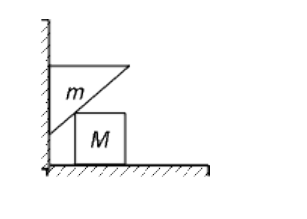
\includegraphics{mainmatter/kinem1.PNG}
        \caption{}
        \label{fig:wedge}
    \end{figure}
    \item A rope of length L and of mass M is suspended on the ends of the points O and O$\prime$ of a horizontal roof as shown in the figure \ref{fig:roof}. If the distance from the ceiling to the lowest point of the string is H, what is the tension in the rope at the lowest point of this?
    \hfill \textsl{(CoPhO)}
    \begin{figure}[htp]
        \centering
        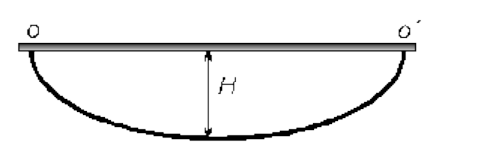
\includegraphics{mainmatter/newt1.PNG}
        \caption{}
        \label{fig:roof}
    \end{figure}
    \item A support mass M is placed on a flat table. Priyani hangs a sphere of mass m by a string of length L and negligible mass. The yarn is separated by a small angle and released. Draw the graph of velocity versus time support. Consider the collision between the sphere and a perfectly elastic.
    \begin{figure}[htp]
        \centering
        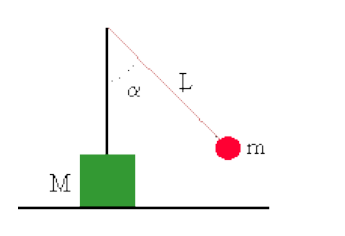
\includegraphics{mainmatter/newt2.PNG}
        \caption{}
        \label{fig:my_label}
    \end{figure}
    
    \item Two particles of mass \textit{m} each are tied at the ends of a light string of length \textit{2a}. The whole system is kept on a frictionless horizontal surface with the string held tight so that each mass is at a distance 'a' from the center 'P' (as shown in the figure). Now, the mid-point of the string is pulled vertically upwards with a small but constant force \textit{F}. As a result, the particles move towards each other on the surface. What is the magnitude of acceleration when the separation between them is 2x. \hfill \textsl{(IIT)}\\
\textsc{Solution:} $\dfrac{Fx}{2m \sqrt{a^2- x^2}}$ 

    \item Two stacks of 20 books each on the ground have to be arranged into a single stack of 40 books. Each of them is d = 2 cm thick and has a mass of 1 kg. What work do we have to perform to move the books? \hfill \textsl{(IIT JEE)}
    \\
    Answer: 80 J 
    
    \item 
\end{enumerate}